\chapter{Experimental Setup and Results}
\label{ch:results}

This chapter evaluates the proposed CEV/IAV closed-loop RAG framework across three decoder-only LLM backbones: \textbf{Mistral-7B-Instruct-v0.2}, \textbf{LLaMA-3-8B-Instruct}, and \textbf{Qwen3-8B}. The experiments answer four questions: (1)~Can CEV and IAV probes reliably detect hallucination on a RAGTruth validation split? (2)~Does probability-level fusion improve over either signal alone? (3)~Does the closed-loop controller reduce delivered hallucination risk relative to vanilla RAG? (4)~Do the probes transfer out of domain?

%% -------------------------------------------------
\section{Experimental Setup}
\label{sec:experimental_setup}

All experiments use Google Colab A100 (40\,GB) with FP16 inference. The probes are trained on extracted activations from the frozen backbone; the backbone weights are never modified. Each backbone's probes, thresholds, and fusion weights are calibrated independently on a stratified RAGTruth validation split.

%% -------------------------------------------------
\section{Dataset Overview}
\label{sec:dataset_overview}

\begin{table}[!htb]
\centering
\caption{Dataset roles in the experimental pipeline.}
\label{tab:dataset_roles}
\small
\begin{tabular}{@{}l r l c c c p{3.5cm}@{}}
\toprule
\textbf{Dataset} & \textbf{Samples} & \textbf{Role} & \textbf{Train?} & \textbf{Retrieval?} & \textbf{Eval?} & \textbf{Purpose} \\
\midrule
RAGTruth-18K & 15{,}090 + 3{,}058 & Probe supervision & Yes & No & Val split & Train/validate probes \\
SQuAD v1.1 (FAISS) & 25{,}000 & Retrieval KB & No & Yes & No & Build FAISS index \\
SQuAD v1.1 (F1) & 10{,}570 & Utility check & No & No & Optional & Token-level F1 \\
HaluEval-QA & 10{,}000 & OOD benchmark & No & No & Yes & Cross-domain transfer \\
HalluRAG & 1{,}098 & Supplementary & Mistral & No & No & Sentence-level examples \\
\bottomrule
\end{tabular}
\end{table}

\subsection{RAGTruth-18K: Primary Probe Supervision}
\label{sec:ragtruth}

RAGTruth~\cite{wu2024ragtruth} provides response-level hallucination labels for RAG-generated text across multiple tasks. The study uses the processed binary label convention:
\begin{itemize}
    \item $y = 0$: Grounded / supported by retrieved context
    \item $y = 1$: Hallucinated / unsupported or contradictory
\end{itemize}

\subsection{SQuAD v1.1: Retrieval Corpus and Operational QA Source}
\label{sec:squad}

SQuAD v1.1~\cite{rajpurkar2016squad} serves dual purposes: (1)~its 25{,}000 training-set contexts form the FAISS retrieval index, and (2)~its validation QA pairs provide the operational queries for closed-loop evaluation.

\subsection{HaluEval-QA: Out-of-Distribution Evaluation}
\label{sec:halueval_dataset}

HaluEval~\cite{li2023halueval} provides paired correct and hallucinated answers. The trained probe scores both, and AUROC measures separation quality.

\subsection{HalluRAG: Mistral-Specific Supplementary Data}
\label{sec:hallurag}

HalluRAG~\cite{frohling2024hallurag} provides sentence-level hallucination labels for Mistral-generated RAG responses.

%% -------------------------------------------------
\section{Dataset Merging and Split Protocol}
\label{sec:split_protocol}

\begin{table}[!htb]
\centering
\caption{Dataset summary.}
\label{tab:dataset_summary}
\small
\begin{tabular}{@{}lrlll@{}}
\toprule
\textbf{Dataset} & \textbf{Samples} & \textbf{Role} & \textbf{Models} & \textbf{Source} \\
\midrule
RAGTruth-18K & 15{,}090 + 3{,}058 & Probe supervision & All & \cite{wu2024ragtruth} \\
SQuAD v1.1 (FAISS) & 25{,}000 & Retrieval KB & All & \cite{rajpurkar2016squad} \\
SQuAD v1.1 (F1) & 10{,}570 & Utility eval & All & \cite{rajpurkar2016squad} \\
HaluEval-QA & 10{,}000 & OOD AUROC & All & \cite{li2023halueval} \\
HalluRAG & 1{,}098 & Supplementary & Mistral only & \cite{frohling2024hallurag} \\
\bottomrule
\end{tabular}
\end{table}

%% -------------------------------------------------
\section{Probe Training Details}
\label{sec:probe_training_details}

\subsection{Loss Function and Class-Weight Calculation}
\label{sec:loss_function}

The probes are trained as binary classifiers: $y \in \{0, 1\} = \{\text{grounded}, \text{hallucinated}\}$. The training loss is class-weighted cross-entropy with label smoothing:
\begin{equation}
    \mathcal{L} = -\sum_{c \in \{0,1\}} w_c \cdot \tilde{y}_c \cdot \log\bigl(\text{softmax}(\mathbf{z})_c\bigr)
    \label{eq:loss}
\end{equation}
where $w_c$ is the class weight and $\tilde{y}_c$ is the smoothed target label.

With approximately \textbf{8{,}369 grounded} and \textbf{6{,}721 hallucinated} examples ($N = 15{,}090$ total), the inverse-frequency weights are:
\begin{align}
    w_{\text{grounded}} &= \frac{15{,}090}{2 \times 8{,}369} = 0.902 \\[4pt]
    w_{\text{hallucinated}} &= \frac{15{,}090}{2 \times 6{,}721} = 1.122
\end{align}

\subsection{Learning-Rate Explanation}
\label{sec:lr_explanation}

\begin{table}[!htb]
\centering
\caption{Learning-rate settings.}
\label{tab:lr_settings}
\begin{tabular}{@{}lll@{}}
\toprule
\textbf{Backbone} & \textbf{Learning Rate} & \textbf{Rationale} \\
\midrule
Mistral-7B-Instruct-v0.2 & $3 \times 10^{-4}$ & Conservative; format-sensitive activations \\
LLaMA-3-8B-Instruct      & $1 \times 10^{-3}$ & Faster convergence; stable activations \\
Qwen3-8B                  & $1 \times 10^{-3}$ & Faster convergence; strong validation signal \\
\bottomrule
\end{tabular}
\end{table}

%% -------------------------------------------------
\section{Threshold Selection and Deployment Calibration}
\label{sec:threshold_selection}

\begin{table}[!htb]
\centering
\caption{Deployment thresholds.}
\label{tab:deploy_thresholds}
\begin{tabular}{@{}lccp{5cm}@{}}
\toprule
\textbf{Backbone} & $\theta_{\text{hallu}}$ & $\theta_{\text{abs}}$ & \textbf{Interpretation} \\
\midrule
Mistral-7B & 0.62 & 0.75 & Conservative; avoids excessive false positives \\
Qwen3-8B   & 0.55 & 0.72 & Lower threshold; stronger score separation \\
LLaMA-3-8B & 0.60 & 0.78 & Higher abstention; reduces over-refusal \\
\bottomrule
\end{tabular}
\end{table}

%% -------------------------------------------------
\section{Primary RAGTruth Validation Results}
\label{sec:primary_results}

\begin{table}[!htb]
\centering
\caption{RAGTruth validation results.}
\label{tab:ragtruth_results}
\begin{tabular}{@{}lcccc@{}}
\toprule
\textbf{Backbone} & \textbf{CEV AUROC} & \textbf{IAV AUROC} & \textbf{Fused AUROC} & \textbf{Mean Acc.} \\
\midrule
Mistral-7B-Instruct-v0.2 & 0.8474 & 0.8474 & 0.8596 & 0.7806 \\
Qwen3-8B                  & \textbf{0.8763} & \textbf{0.8709} & \textbf{0.8808} & \textbf{0.7995} \\
LLaMA-3-8B-Instruct      & 0.8579 & 0.8622 & 0.8689 & 0.7822 \\
\bottomrule
\end{tabular}
\end{table}

\begin{figure}[!htb]
    \centering
    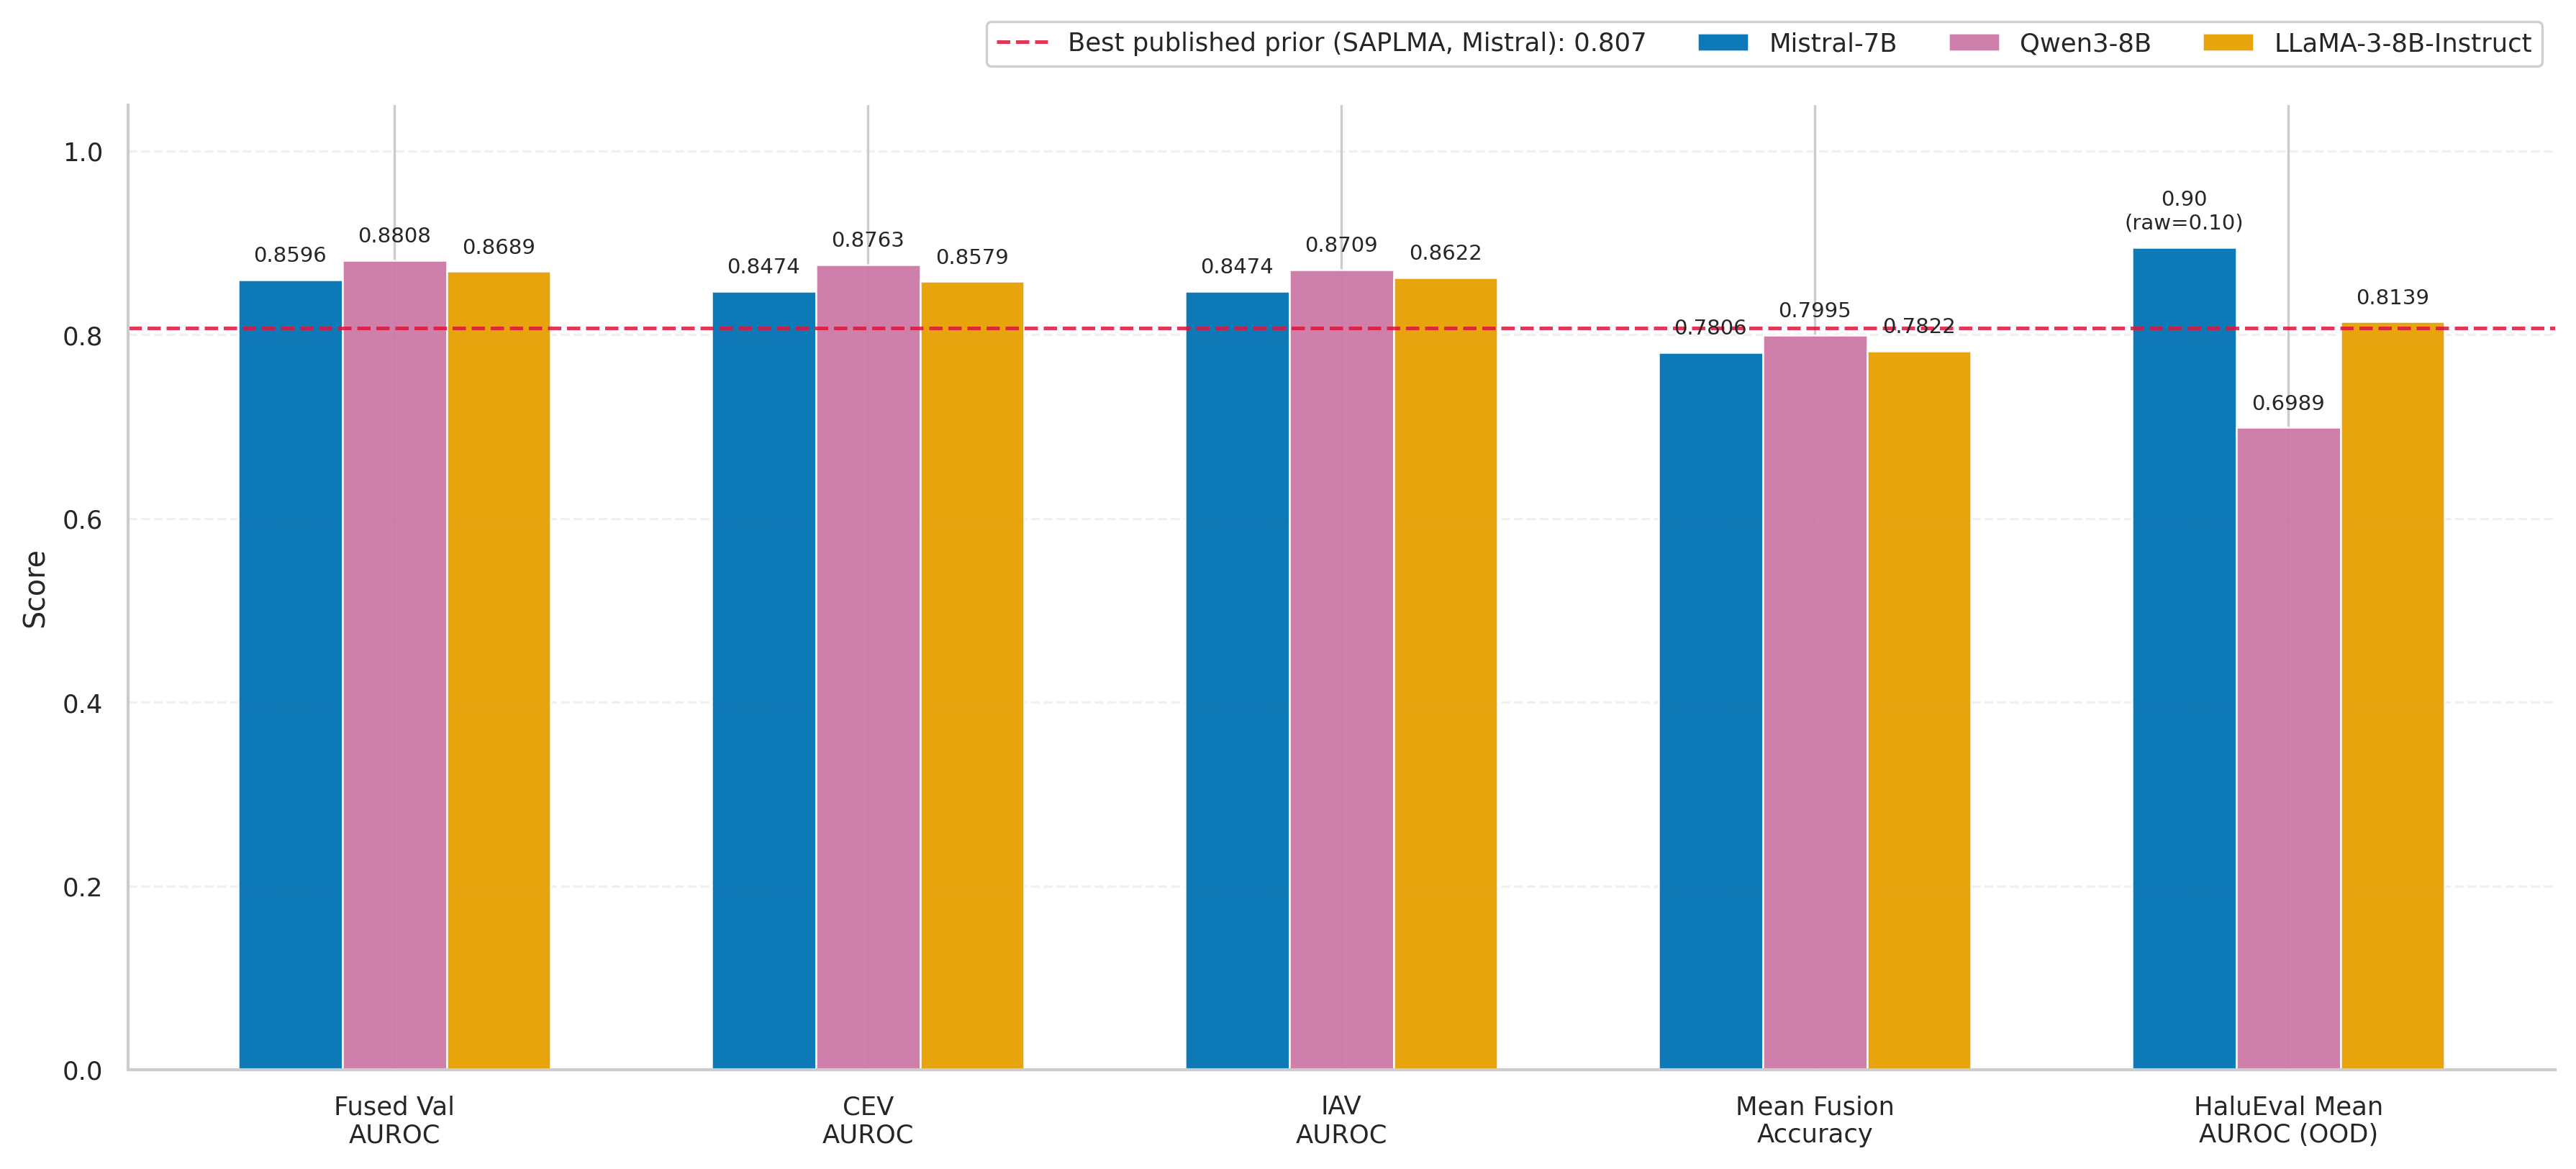
\includegraphics[width=0.90\textwidth]{Images/our_models_multi_metric.png}
    \caption[Cross-model probe performance.]{Cross-model probe performance across validation and OOD metrics. Fused AUROC, CEV AUROC, IAV AUROC, mean fusion accuracy, and HaluEval mean AUROC compared across the three backbones.}
    \label{fig:multi_metric}
\end{figure}

%% -------------------------------------------------
\section{Probe Score Distributions}
\label{sec:score_distributions}

\begin{figure}[!htb]
    \centering
    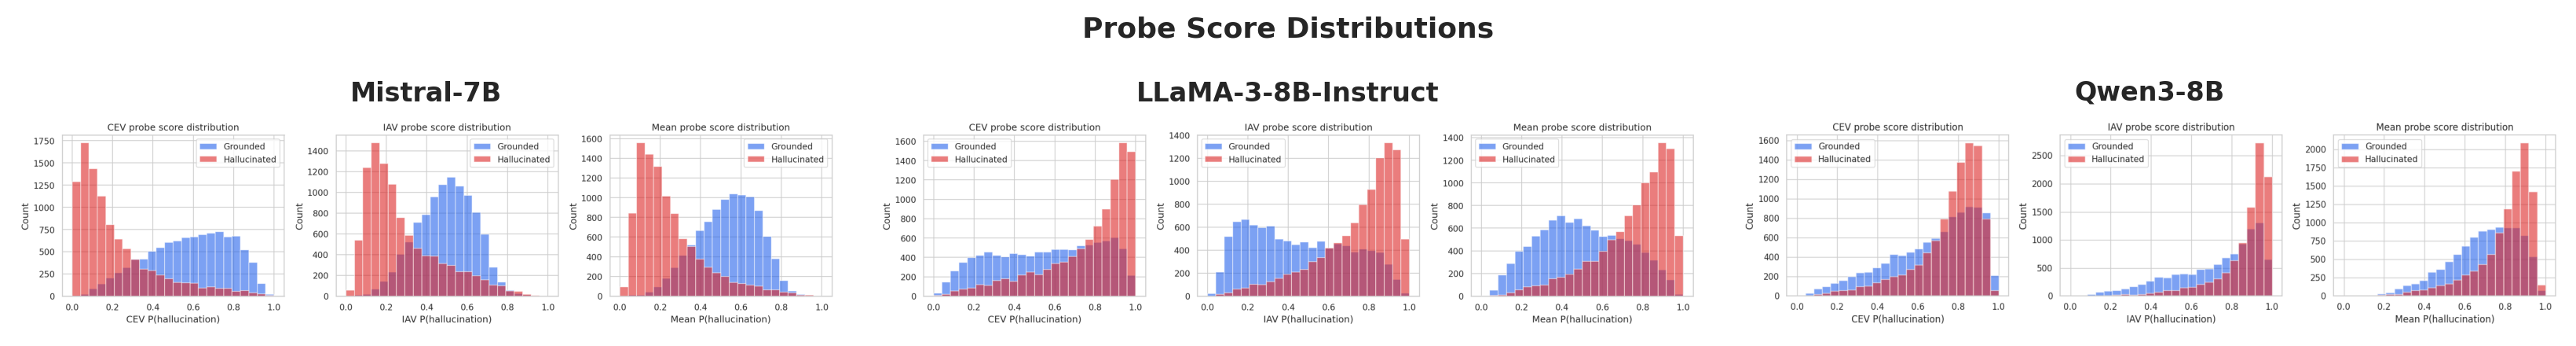
\includegraphics[width=0.90\textwidth]{Images/probe_score_histograms_grid.png}
    \caption[Probe score distributions.]{Probe score distributions for grounded and hallucinated examples. The overlap between distributions indicates the difficulty of perfect binary separation; partial overlap is expected because hallucination is a graded phenomenon.}
    \label{fig:score_histograms}
\end{figure}

%% -------------------------------------------------
\section{Baseline Comparison on RAGTruth}
\label{sec:baseline_comparison}

\begin{table}[!htb]
\centering
\caption{Comparison with RAGTruth hallucination-detection baselines.}
\label{tab:baselines}
\small
\begin{tabular}{@{}l l c cc@{}}
\toprule
\textbf{Method} & \textbf{Signal Type} & \textbf{CL?} & \textbf{Mistral} & \textbf{LLaMA} \\
\midrule
SelfCheckGPT~\cite{manakul2023selfcheckgpt}   & Multi-sample consistency & No & 0.568 & 0.534 \\
EigenScore/INSIDE~\cite{chen2024inside}         & Hidden-state spectral    & No & 0.564 & 0.600 \\
RefChecker~\cite{hu2024refchecker}              & Reference-based          & No & 0.602 & 0.572 \\
P(True)~\cite{kadavath2022language}             & Output confidence        & No & 0.753 & 0.541 \\
Focus~\cite{focus2024}                          & Uncertainty scoring      & No & 0.780 & 0.526 \\
Perplexity/entropy~\cite{varshney2023stitch}    & Output probability       & No & 0.620 & 0.713 \\
LN-Entropy~\cite{varshney2023stitch}            & Output uncertainty       & No & 0.761 & 0.707 \\
ReDeEP~\cite{redeep2024}                        & Attention + FFN          & Partial & 0.762 & 0.750 \\
LUMINA~\cite{lumina2024}                         & Context--knowledge       & No & 0.769 & 0.745 \\
SAPLMA~\cite{azaria2023saplma}                  & Hidden-state probe       & No & 0.807 & 0.760 \\
\midrule
\textbf{Ours: Fused CEV/IAV}                    & \textbf{Residual + FFN}  & \textbf{Yes} & \textbf{0.8596} & \textbf{0.8689} \\
\bottomrule
\end{tabular}
\end{table}

\begin{figure}[!htb]
    \centering
    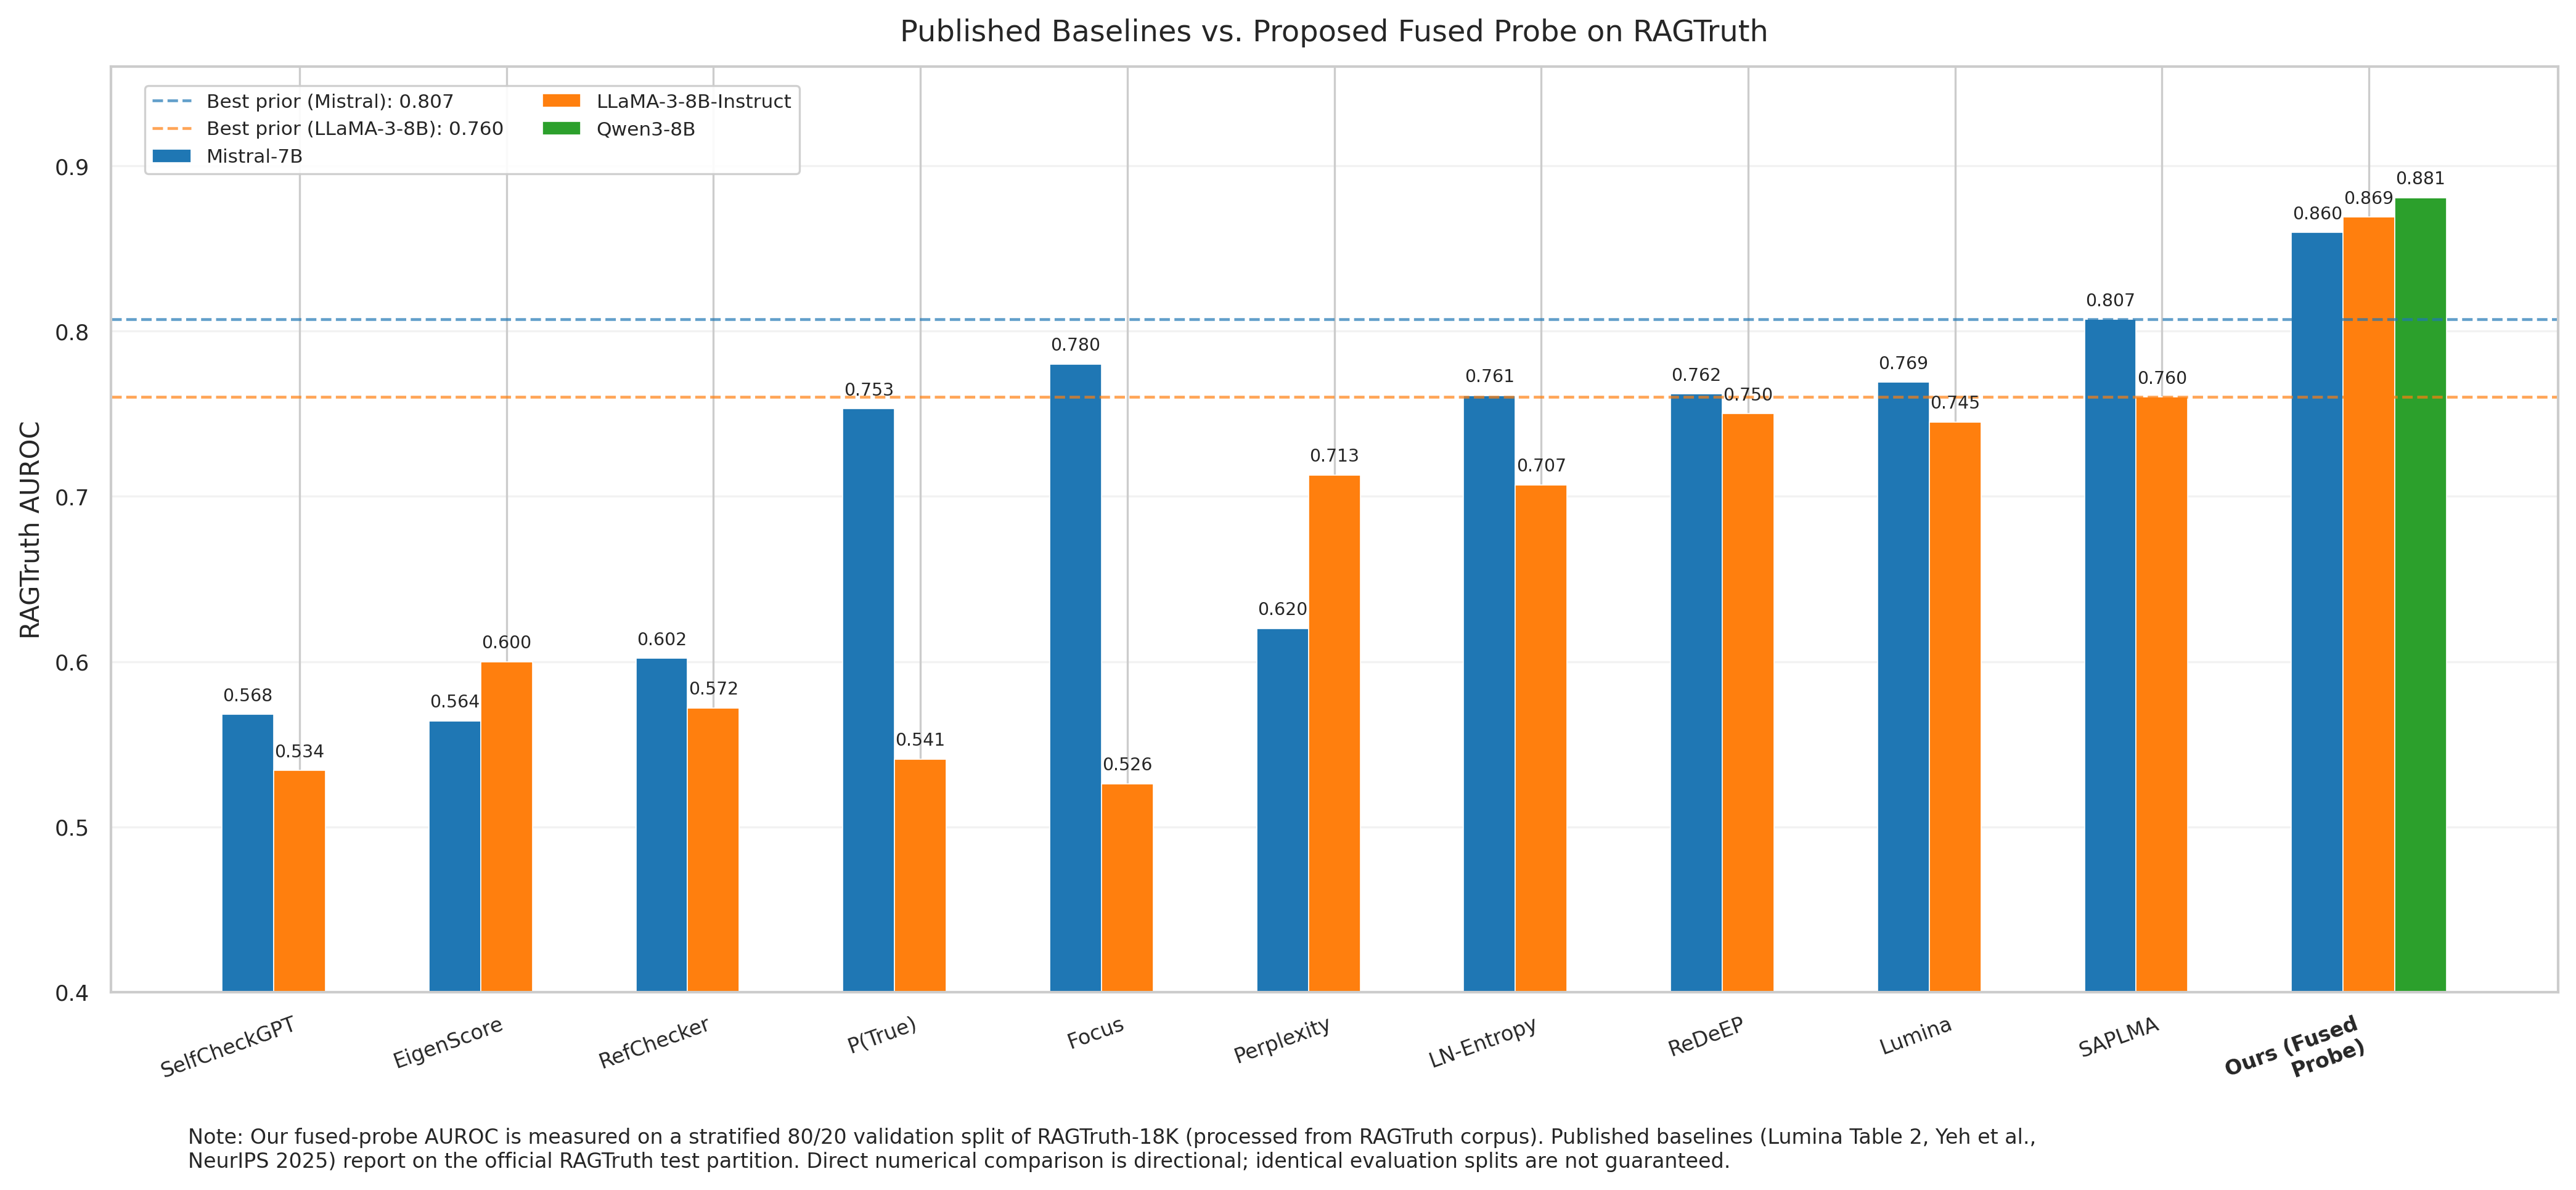
\includegraphics[width=0.90\textwidth]{Images/compare_prior_work_ragtruth_paper_style.png}
    \caption[Baselines vs.\ proposed probe on RAGTruth AUROC.]{Published baselines vs.\ proposed fused CEV/IAV probe on RAGTruth AUROC. The proposed method achieves the highest AUROC on both Mistral and LLaMA backbones while being the only method with closed-loop capability.}
    \label{fig:baselines}
\end{figure}

%% -------------------------------------------------
\section{Vanilla RAG vs.\ Closed-Loop RAG}
\label{sec:vanilla_vs_cl}

\begin{table}[!htb]
\centering
\caption{Vanilla RAG vs.\ closed-loop RAG comparison.}
\label{tab:vanilla_vs_cl}
\begin{tabular}{@{}lcccrr@{}}
\toprule
\textbf{Backbone} & \textbf{Vanilla Proxy} & \textbf{CL Proxy} & \textbf{Reduction} & \textbf{Accept} & \textbf{Abstain} \\
\midrule
Mistral-7B  & 0.3301 & \textbf{0.1068} & 67.6\% & 62\% & 38\% \\
Qwen3-8B    & 0.5388 & 0.1116          & \textbf{79.3\%} & 42\% & 58\% \\
LLaMA-3-8B  & 0.3321 & 0.1824          & 45.1\% & \textbf{90\%} & 10\% \\
\bottomrule
\end{tabular}
\end{table}

\begin{figure}[!htb]
    \centering
    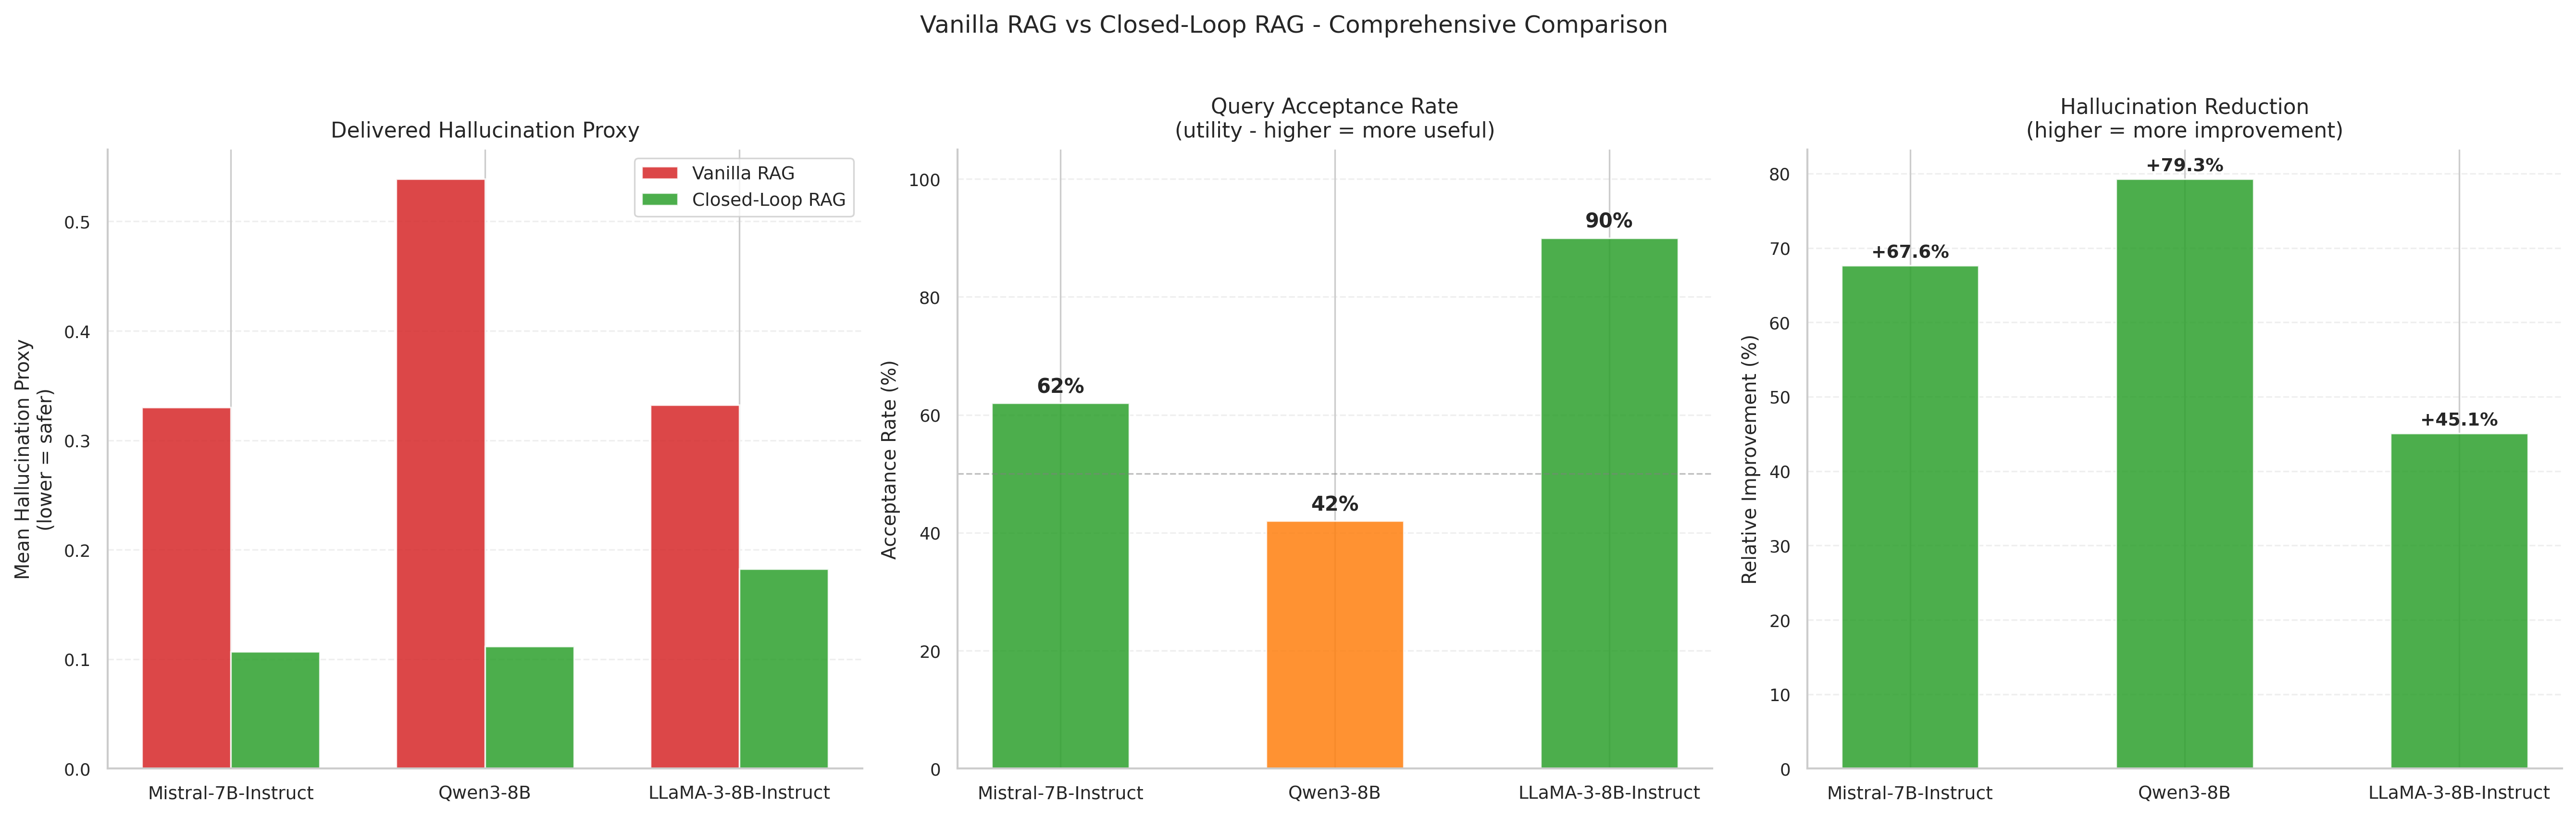
\includegraphics[width=0.90\textwidth]{Images/vanilla_vs_closedloop_comparison.png}
    \caption[Vanilla RAG vs.\ closed-loop RAG comparison.]{Vanilla RAG vs.\ closed-loop RAG: delivered hallucination proxy, acceptance rate, and relative reduction across the three backbones.}
    \label{fig:vanilla_vs_cl}
\end{figure}

\textbf{Interpretation.} The closed-loop controller reduces delivered hallucination risk for all three backbones; the per-backbone safety--utility profiles (Mistral balanced, Qwen conservative, LLaMA permissive) are discussed in Section~\ref{sec:safety_utility}.

\textbf{Threats to validity (proxy metric).} These reductions are measured with the system's own calibrated probe score rather than with human or external judgments---the metric is therefore partly self-referential. Three specific caveats apply: (i)~the proxy cannot catch the failure mode of Section~\ref{sec:illustrative_examples}, where confident but unsupported extractions are scored as low-risk; (ii)~the 100-query sample at one seed carries sampling noise; and (iii)~the RE-RETRIEVE branch was rarely exercised. These caveats are formalized as Limitations~6--8 in Section~\ref{sec:limitations}.

%% -------------------------------------------------
\section{Ablation Study: CEV, IAV, and Fusion}
\label{sec:ablation}

\begin{table}[!htb]
\centering
\caption{Probe ablation accuracy.}
\label{tab:ablation}
\begin{tabular}{@{}lcccc@{}}
\toprule
\textbf{Backbone} & \textbf{CEV-only} & \textbf{IAV-only} & \textbf{Mean-fusion} & \textbf{Best} \\
\midrule
Mistral-7B  & 0.772 & 0.778 & \textbf{0.781} & Fusion \\
Qwen3-8B    & 0.799 & 0.793 & \textbf{0.800} & Fusion \\
LLaMA-3-8B  & \textbf{0.789} & 0.782 & 0.782 & CEV \\
\bottomrule
\end{tabular}
\end{table}

\begin{figure}[!htb]
    \centering
    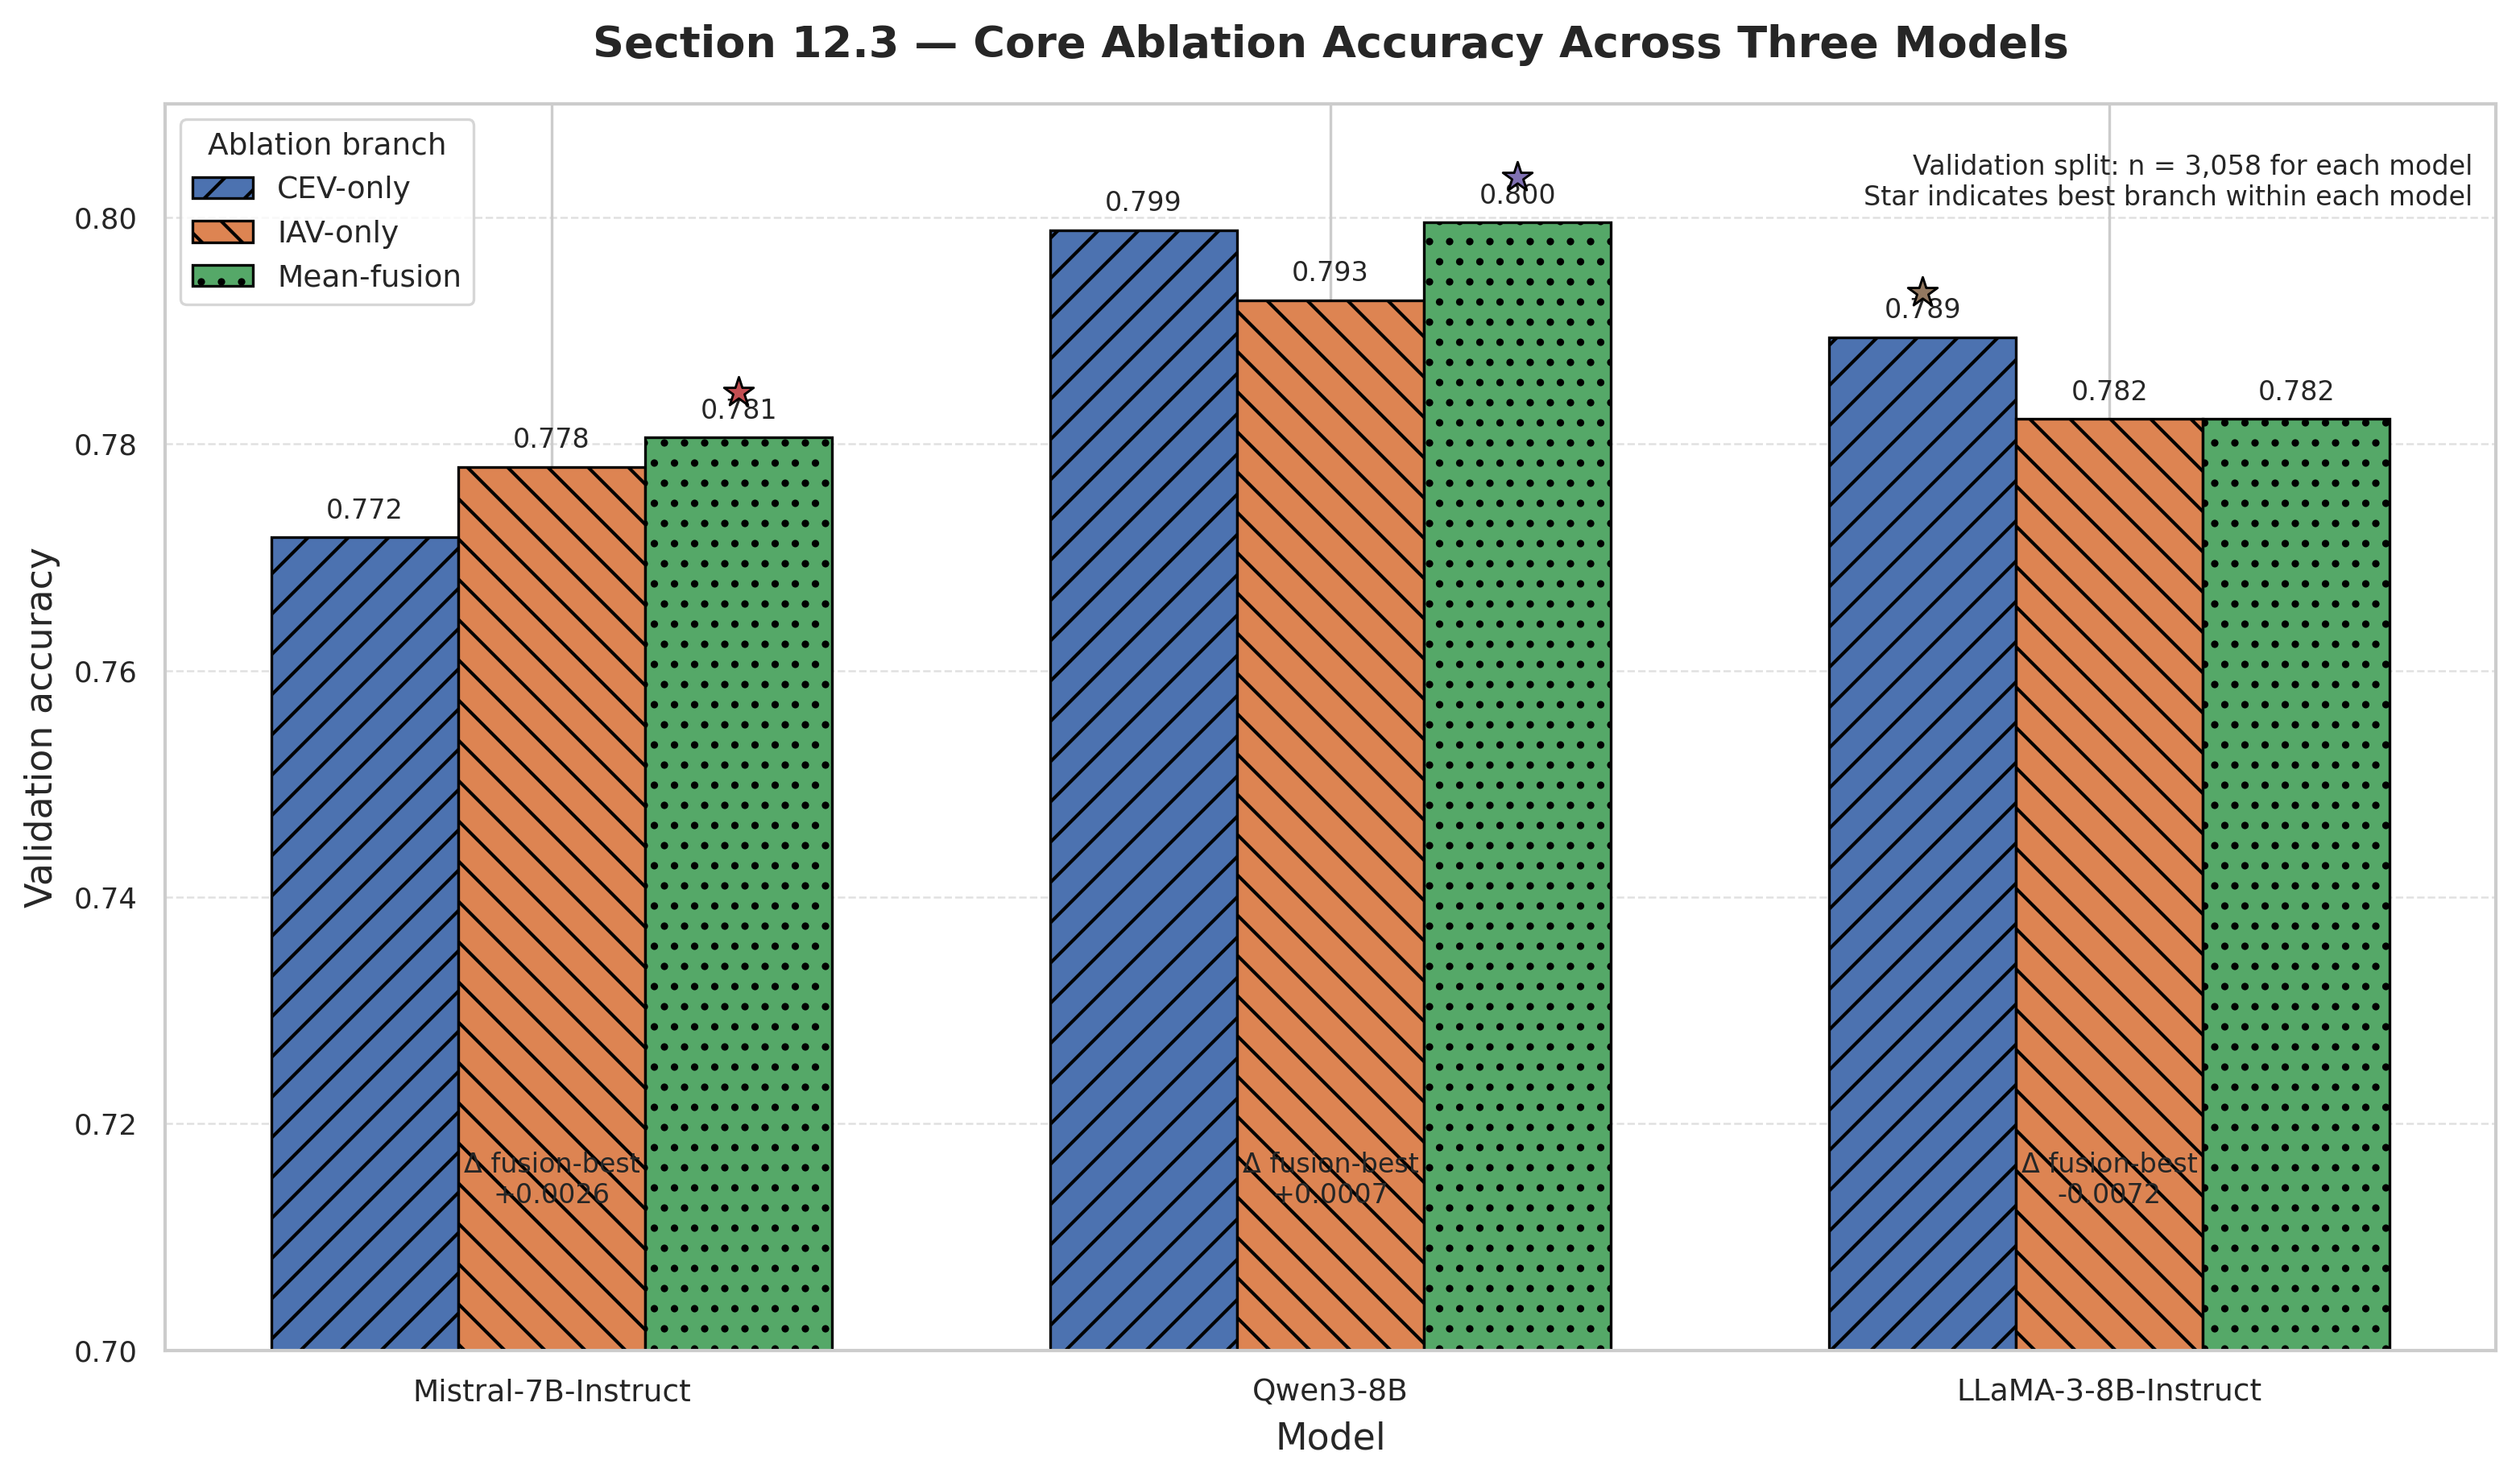
\includegraphics[width=0.85\textwidth]{Images/section12_3_core_ablation_accuracy_comparison.png}
    \caption[Ablation: CEV-only, IAV-only, and mean-fusion accuracy.]{Ablation comparison across CEV-only, IAV-only, and mean-fusion scores for the three backbones.}
    \label{fig:ablation}
\end{figure}

%% -------------------------------------------------
\section{HaluEval Out-of-Distribution Analysis}
\label{sec:halueval_ood}

\begin{table}[!htb]
\centering
\caption{HaluEval out-of-distribution AUROC.}
\label{tab:halueval_ood}
\small
\begin{tabular}{@{}l l l l l@{}}
\toprule
\textbf{Backbone} & \textbf{CEV} & \textbf{IAV} & \textbf{Mean/Fused} & \textbf{Interpretation} \\
\midrule
Mistral-7B & 0.106 / 0.894 adj. & 0.175 / 0.825 adj. & 0.105 / 0.895 adj. & Polarity inversion \\
Qwen3-8B   & 0.604 & 0.723 & 0.699 & Aligned transfer \\
LLaMA-3-8B & 0.740 & 0.816 & \textbf{0.814} & Best aligned \\
\bottomrule
\end{tabular}
\end{table}

\begin{figure}[!htb]
    \centering
    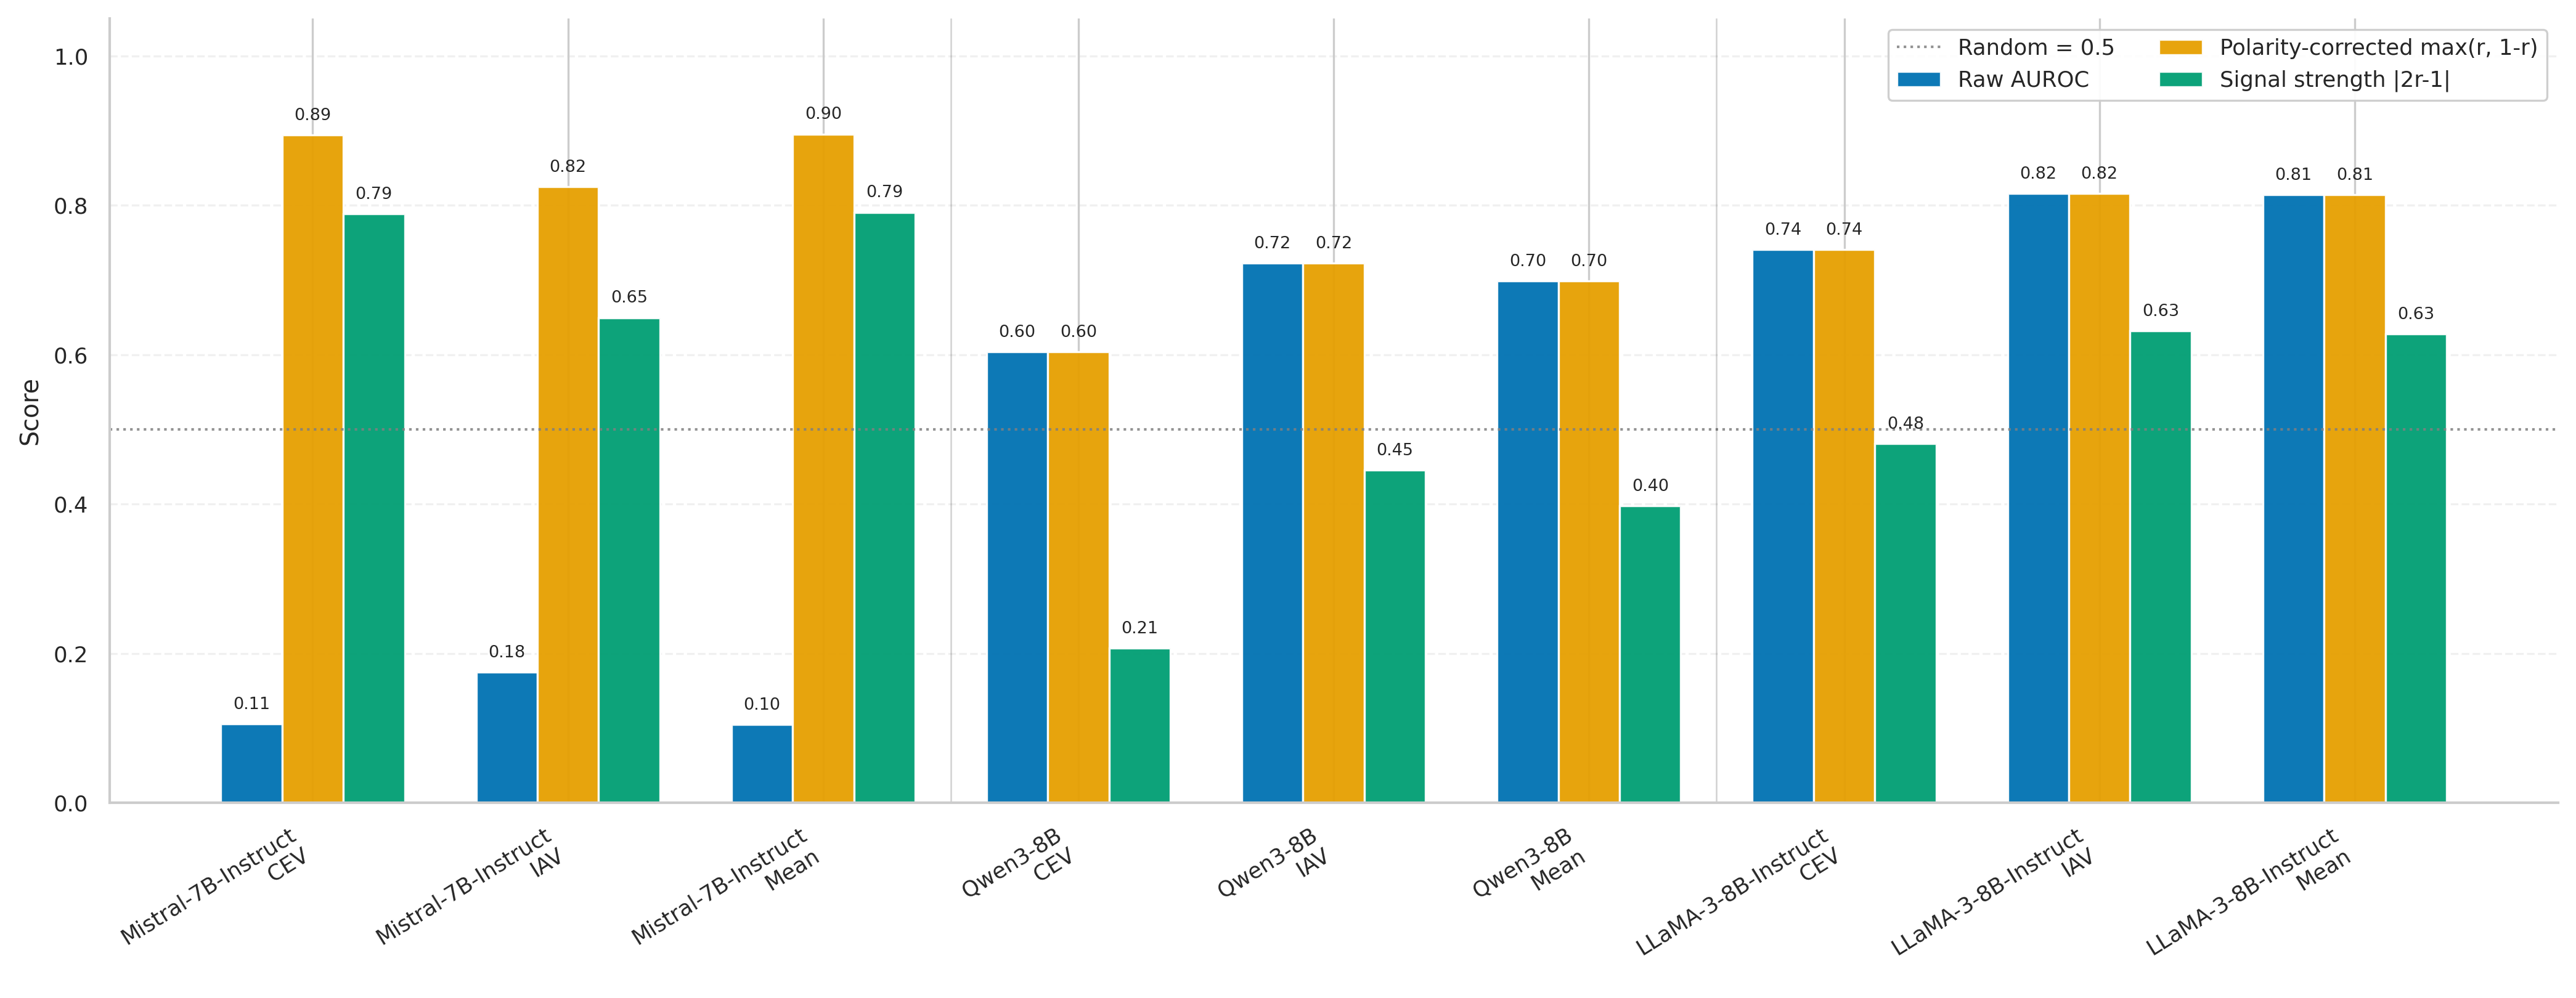
\includegraphics[width=0.90\textwidth]{Images/halueval_three_column.png}
    \caption[HaluEval OOD analysis.]{HaluEval raw AUROC, orientation-adjusted AUROC, and signal strength. Mistral shows strong polarity inversion; LLaMA and Qwen preserve aligned transfer.}
    \label{fig:halueval}
\end{figure}

%% -------------------------------------------------
\section{Nine-Query Live Demonstration}
\label{sec:nine_query_demo}

\begin{table}[!htb]
\centering
\caption{Nine-query outcomes per backbone (fused score in parentheses).}
\label{tab:nine_query}
\footnotesize
\begin{tabularx}{\textwidth}{@{}c p{3.5cm} X X X@{}}
\toprule
\textbf{\#} & \textbf{Query Type} & \textbf{Mistral-7B} & \textbf{Qwen3-8B} & \textbf{LLaMA-3-8B} \\
\midrule
1 & Author (answerable) & ACCEPT (0.59) & ABSTAIN (0.72) & ACCEPT (0.07) \\
2 & Westphalia (answerable) & ACCEPT (0.60) & ACCEPT (0.42) & ACCEPT (0.08) \\
3 & Kelvin (answerable) & ACCEPT (0.42) & ACCEPT (0.33) & ACCEPT (0.19) \\
4 & Breakfast (impossible) & ACCEPT (0.12) & ABSTAIN (0.86) & ACCEPT (0.19) \\
5 & Mars capital (impossible) & ACCEPT (0.17) & REGEN$\times$2$\to$ACCEPT (0.20) & ACCEPT (0.17) \\
6 & Climate (RAG-supported) & ACCEPT (0.34) & ACCEPT (0.38) & ACCEPT (0.47) \\
7 & Shakespeare (subjective) & ACCEPT (0.08) & ACCEPT (0.22) & ACCEPT (0.10) \\
8 & Five planets (answerable) & ACCEPT (0.52) & REGEN$\times$2$\to$ACCEPT (0.51) & ACCEPT (0.11) \\
9 & Atlantis census (nonsensical) & ACCEPT (0.31) & ABSTAIN (0.80) & ACCEPT (0.10) \\
\midrule
\multicolumn{2}{@{}l}{\textbf{Action totals (accept/abstain)}} & \textbf{9 / 0} & \textbf{6 / 3} & \textbf{9 / 0} \\
\bottomrule
\end{tabularx}
\end{table}

%% -------------------------------------------------
\section{Cross-Model Summary}
\label{sec:cross_model_summary}

\begin{table}[!htb]
\centering
\caption{Cross-model comparison (Table~8.13).}
\label{tab:cross_model}
\begin{tabular}{@{}lccc@{}}
\toprule
\textbf{Metric} & \textbf{Mistral-7B} & \textbf{Qwen3-8B} & \textbf{LLaMA-3-8B} \\
\midrule
Fused validation AUROC    & 0.8596 & \textbf{0.8808} & 0.8689 \\
CEV AUROC                 & 0.8474 & \textbf{0.8763} & 0.8579 \\
IAV AUROC                 & 0.8474 & \textbf{0.8709} & 0.8622 \\
Mean-fusion accuracy      & 0.7806 & \textbf{0.7995} & 0.7822 \\
HaluEval mean AUROC (raw) & 0.105 inv. & 0.699 & \textbf{0.814} \\
Vanilla delivered proxy   & 0.3301 & 0.5388 & 0.3321 \\
Closed-loop proxy         & \textbf{0.1068} & 0.1116 & 0.1824 \\
Relative reduction        & 67.6\% & \textbf{79.3\%} & 45.1\% \\
Acceptance rate           & 62\% & 42\% & \textbf{90\%} \\
Nine-query (accept/abstain) & 9/0 & 6/3 & 9/0 \\
Fusion weight (CEV/IAV)   & 0.50/0.50 & 0.60/0.40 & 0.45/0.55 \\
\bottomrule
\end{tabular}
\end{table}
